documentclass[aspectratio=209]{beamer}


\usepackage[T2A]{fontenc}
\usepackage[koi8-r]{inputenc}
\usepackage[english]{babel}
\usepackage{amssymb,amsfonts,amsmath,mathtext}
\usepackage{cite,enumerate,float,indentfirst}


\usetheme{Antibes}
\usecolortheme{crane}


\title{Software project:Developing a decision-making assistant }
\author{Morozova Milena}

\begin{document}

%---------------------------------------------------------
\begin{frame}% первый слайд
\titlepage
\end{frame}
%---------------------------------------------------------
\begin{frame}
\frametitle{Table of Contents}
\tableofcontents
\end{frame}

%---------------------------------------------------------
%---------------------------------------------------------
\section{Introduction}

\begin{frame}
\frametitle{Basic Tasks}
\begin{itemize}
    \item Creating a training sample
    \item Preprocessing training sample
    \item Building and training the model
    \item Testing the Model
\end{itemize}
    \begin{figure}
	    \begin{center}
		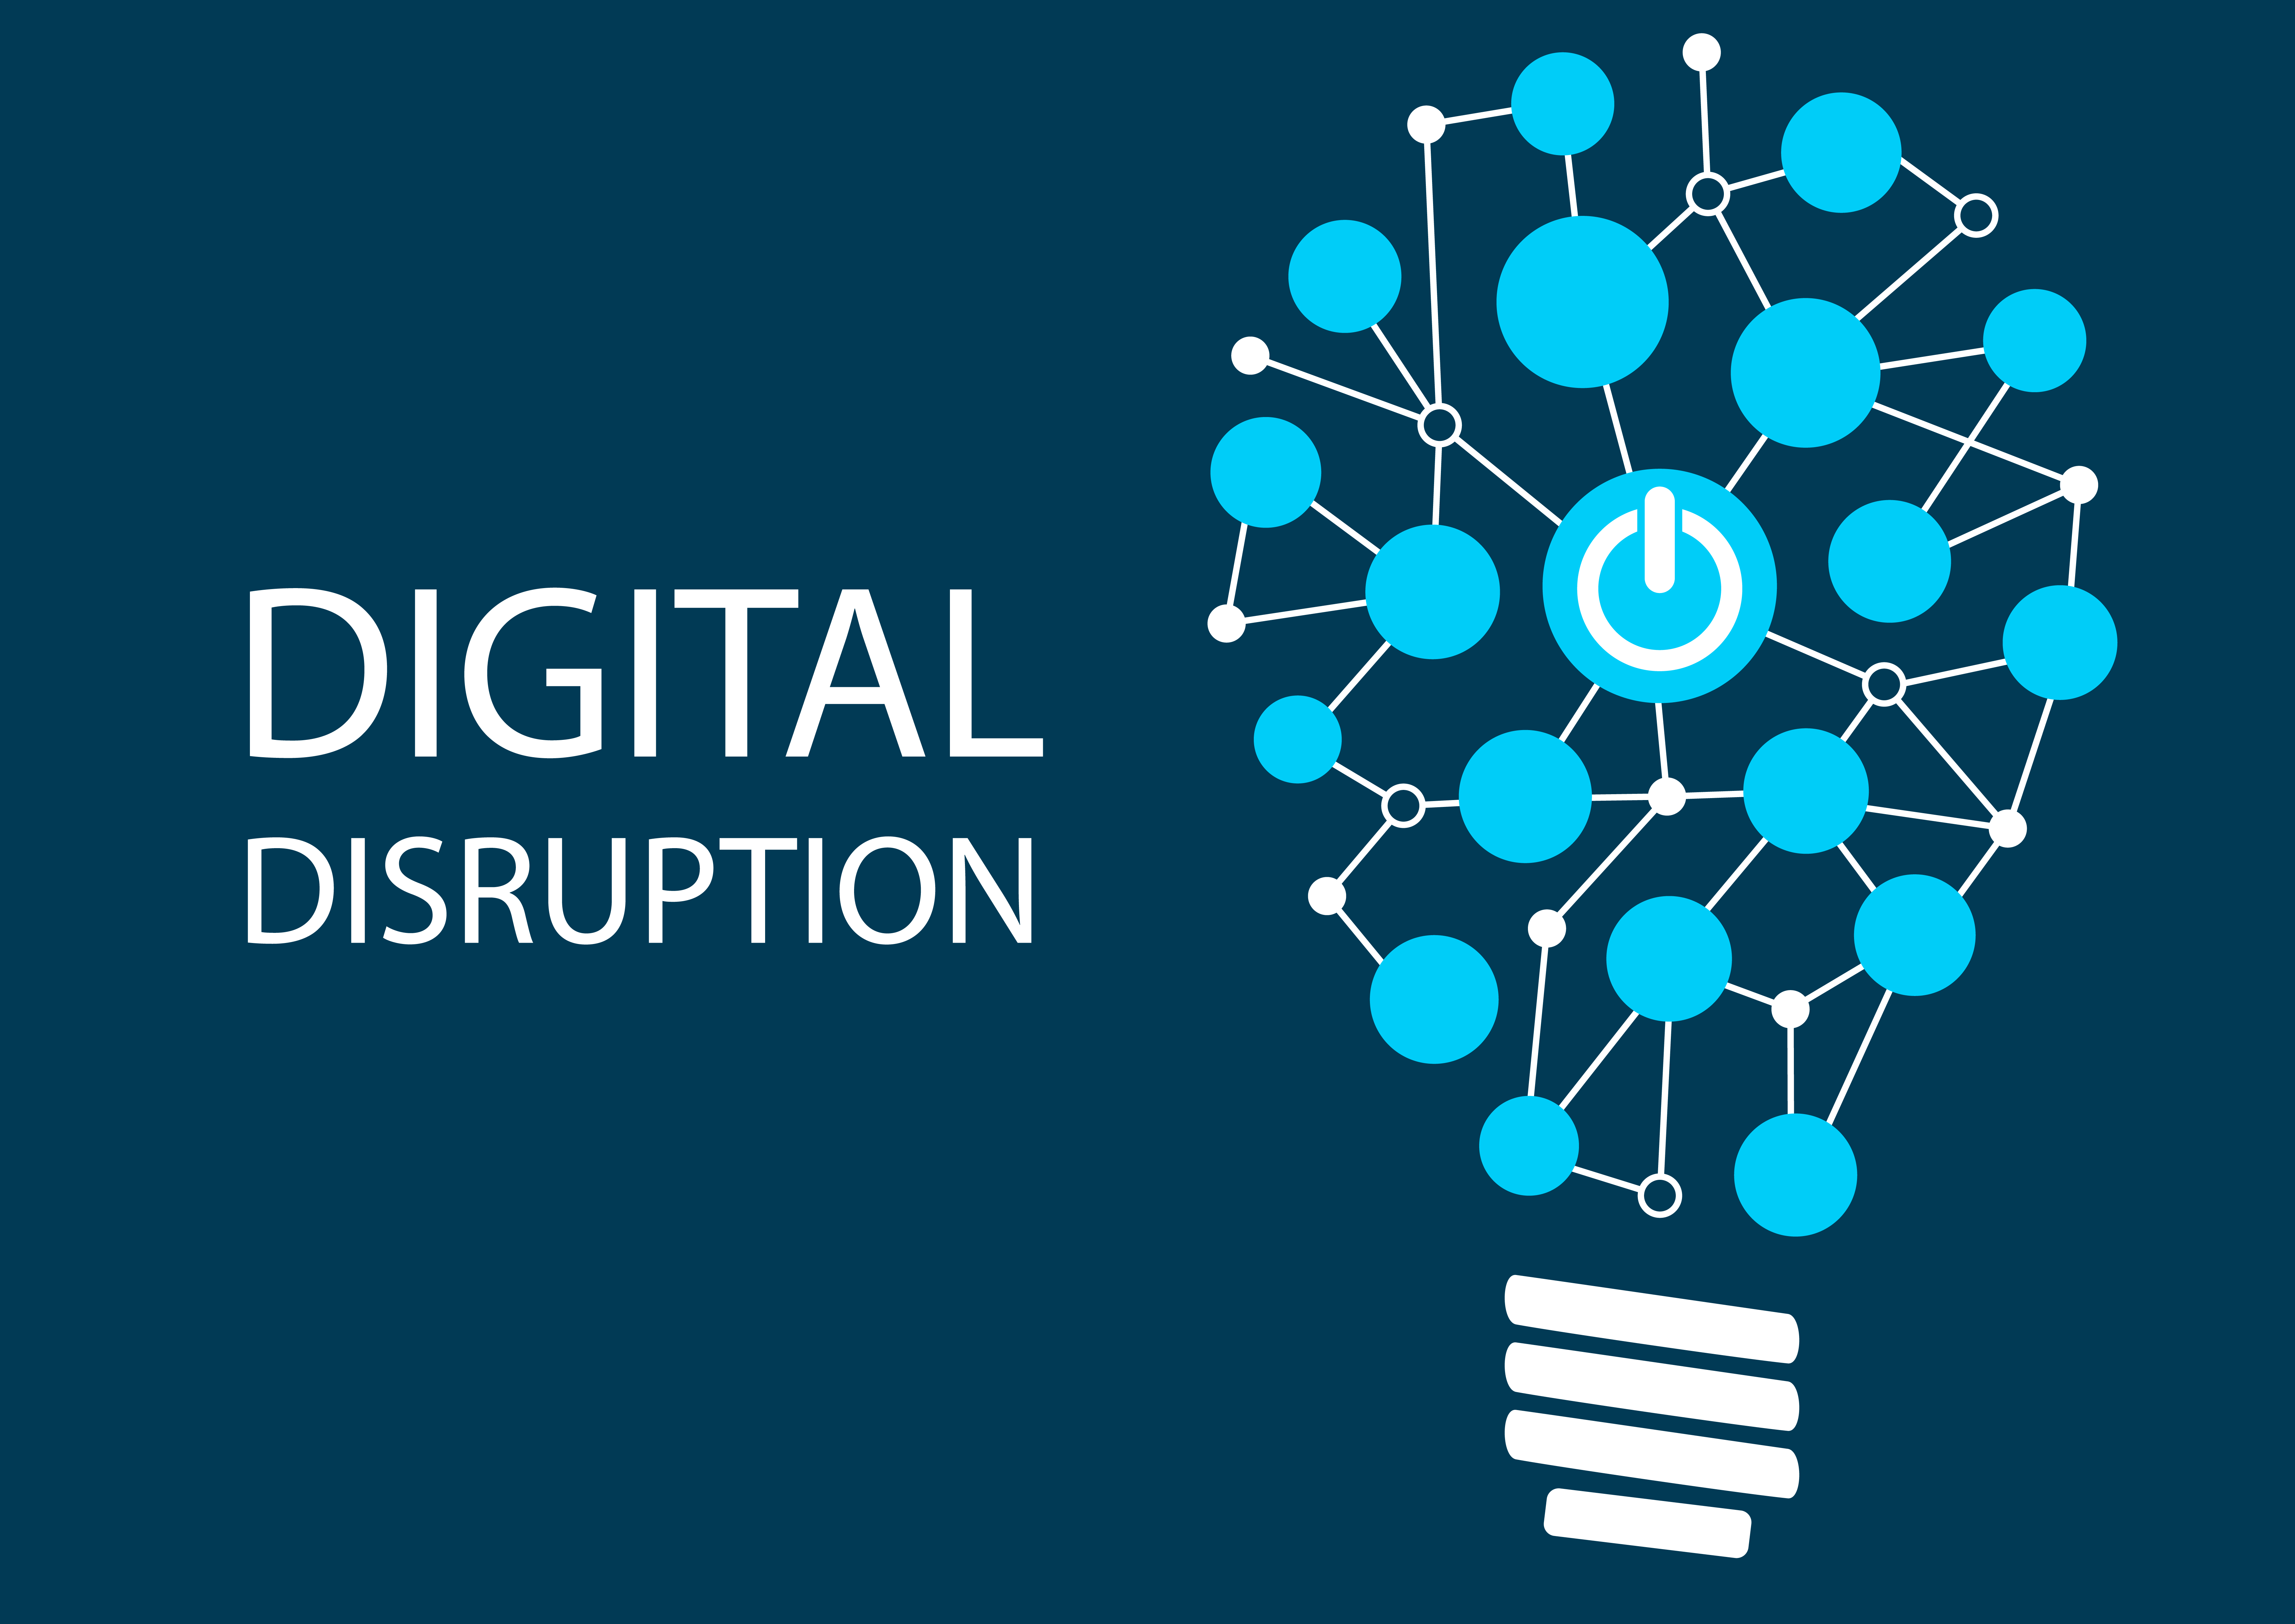
\includegraphics[width=0.5\linewidth]{{images/pict17.jpg}}
	    \end{center}
        \end{figure}
\end{frame}
%---------------------------------------------------------
\begin{frame}
\frametitle{Additional Tasks}
\begin{itemize}
    \item Rating calculation
    \item Creating GUI
    \item Testing the App on different platforms
    \item Setting the application icon
\end{itemize}
    \begin{figure}
	    \begin{center}
		
\includegraphics[width=0.5\linewidth]{{images/pict18.jpg}}
	    \end{center}
    \end{figure}    
\end{frame}
%---------------------------------------------------------
%---------------------------------------------------------

\section{Working with a training sample}


\begin{frame}
\frametitle{Preprocessing the sample}
\begin{columns}
% Column 1
\begin{column}{0.4\textwidth}
Any text data in its raw material form cannot be analyzed by NLP libraries. This data must be cleaned using various data processing techniques.
\end{column}
% Column 2    
\begin{column}{0.6\textwidth}
    \begin{figure}
    \centering
        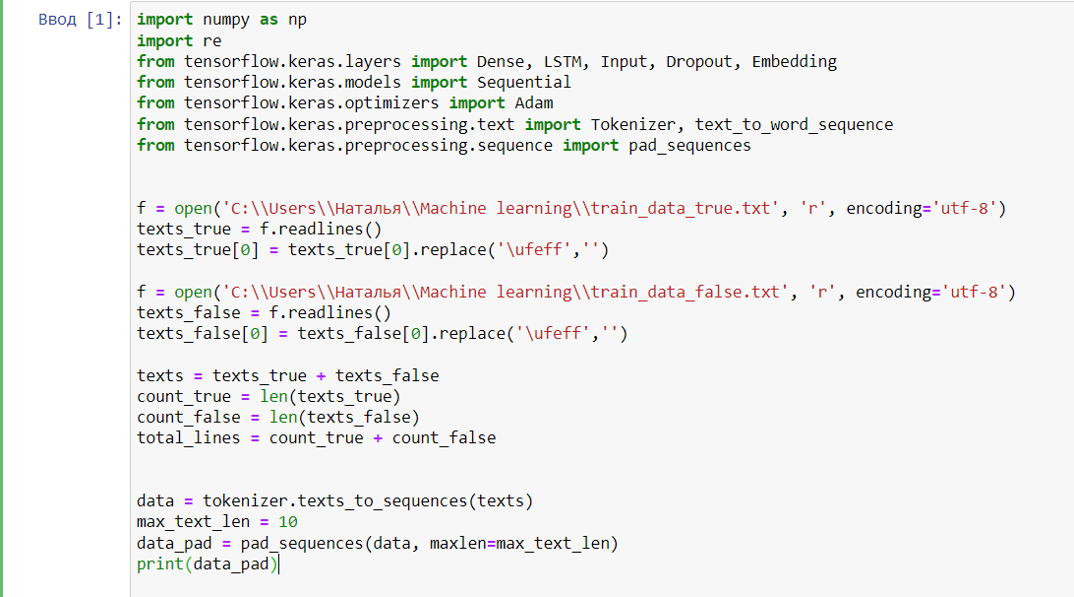
\includegraphics[width=0.9\textwidth]{images/sample1.png}
        \caption{Preprocessing the training sample}
    \end{figure}
\end{column}
\end{columns}
\end{frame}

%---------------------------------------------------------
%---------------------------------------------------------

\section{Building and training the model}

\begin{frame}
Our neural network will have 2 neurons at the output - the upper neuron will be responsible for the positive text, the lower - for the negative. For positive statements at the output, we will require the vector [1.0], respectively for negative - [0.1].

\begin{figure}
\centering
    \begin{subfigure}
        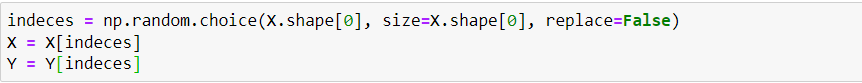
\includegraphics[width=0.5\textwidth]{images/pict7.png}
        \caption{Training}
        \label{fig:nature1}
    \end{subfigure}
    \begin{subfigure}
        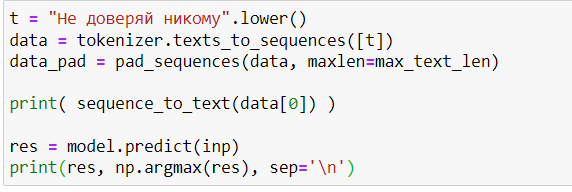
\includegraphics[width=0.5\textwidth]{images/pict11.png}
        \caption{Testing}
        \label{fig:nature2}
    \end{subfigure}
\caption{Working with a mathematical model}
\label{fig:images}
\end{figure}
\end{frame}


%---------------------------------------------------------
%---------------------------------------------------------

\section{List of Sources}

\begin{frame}
\frametitle{Bibliography}
\begin{itemize}
\item Machine Learning, Neural and Statistical Classification 

\url{https://www1.maths.leeds.ac.uk/~charles/statlog/}

\item Cleaning & Preprocessing Text Data for Sentiment Analysis 

\url{https://towardsdatascience.com/}

\item Generating WordClouds in Python Tutorial 

\url{https://www.datacamp.com/tutorial/wordcloud-python}

\item TripAdvisor

\url{https://www.tripadvisor.ru/}

\item Sentiment Analysis of Review Datasets

\url{https://www.researchgate.net/publication}

\item Keras Documentation

\url{https://ru-keras.com/recurrent-layers/}

\end{itemize}
\end{frame}


\end{document}
